\documentclass[11pt]{article}
\usepackage[utf8]{inputenc}
\usepackage[brazil]{babel}
\usepackage{graphicx}
\usepackage{tabularx}
\DeclareGraphicsExtensions{.pdf,.png,.jpg}
\setlength{\topmargin}{-.5in}
\setlength{\textheight}{9in}
\setlength{\oddsidemargin}{.125in}
\setlength{\textwidth}{6.25in}
\usepackage{xcolor,colortbl}
\definecolor{gray}{rgb}{0.85,0.85,0.85}
\definecolor{lightblue}{rgb}{0.75,0.75,0.75}

\begin{document}

  \begin{titlepage}
  
    \centering
    
\includegraphics[width=.5\textwidth]{logo.jpg}

    \vspace{\stretch{1}}
    \large{CURSO SUPERIOR DE TECNOLOGIA EM ANÁLISE E DESENVOLVIMENTO DE SISTEMAS, REDES DE COMPUTADORES E GESTÃO DE TECNOLOGIA DA INFORMAÇÃO}

    \vspace{\stretch{1}}

    \large{BRAUNER SOUZA DE MELLO\\DALMIR DA SILVA}

    \vspace{\stretch{1}}
    \large{\textbf{Graform}}

    \vspace{\stretch{2}}
    \large{PORTO ALEGRE, \\DEZ de 2013}
    
  \end{titlepage}

  \newpage
  \thispagestyle{empty}
  \mbox{}
  \newpage

  \begin{abstract}
    Graform é um sistema de criação e gerenciamento de formulário eletronicos. Diferente das principais solução já existentes no mercado, o Graform possui um
    importante distema de descontinuidade de questões. Baseado em regras aplicadas a cada resposta de uma determinada questão, é possível redirecionar o fluxo das próximas
    questões a serem respondidas. Possibilitando assim, coletar informações mais relevantes do que um questionário apenas sequencial.
  \end{abstract}

  \newpage

  \section{Introdução}

    \paragraph{} \hspace{10pt}
    
    A Stringhini Marketing é uma empresa de marketing com experiência em gestão da operação comercial e do relacionamento com o cliente através do monitoramento de indicadores chave e índices de satisfação. A empresa dá muita importância à inteligência competitiva e procura transformar informação em estratégia e decisão em resultado, agregando valor ao negócio dos clientes.

    \paragraph{} \hspace{10pt}

    Pelo grande número de informações trabalhadas em uma pesquisa de marketing, há uma grande dificuldade em não se ter uma interface amigável de criação e gerenciamento de pesquisas.
    O desenvolvimento dos questionários é diretamente no banco de dados através de scripts, o que gerar um grande risco de inconsistência pela possibilidade de erro humano, a dificuldade de manutenção é muito alta, tornando a personalização de um questionário quase impossível.
    No atual momento a empresa não vê condições de adquirir um software no mercado, por julgar que não atenda em relação aos custos e necessidades específicas de cada projeto.

    \paragraph{} \hspace{10pt}

    O objetivo do projeto é desenvolver uma ferramenta web para criação e gerenciamento de pesquisas, com uma interface amigável e usual para os clientes. Com o desenvolvimento deste software a empresa permitirá autonomia aos clientes, pois os mesmos terão condições de desenvolver suas pesquisas conforme sua necessidade, bem como possibilitará a sua equipe tenha condições de focar apenas na inteligência do negócio e não mais ma operação.

  \newpage

  \section{Sistema}

    \subsection{Definição}

      \paragraph{} \hspace{10pt}
      
      O projeto em questão trata-se de um sistema de desenvolvimento de questionários eletrônicos e apresenta as seguintes características:

      \begin{enumerate}
        \item Provê uma interface web para manipulação dos formulários;
        \item Possibilita a criação de dois tipos distintos de formulários:
          \begin{enumerate}
            \item Condicional: A sequência de perguntas a ser respondidas pode variar de acordo com as respostas;
            \item Contínuo: Possui sequência estática de perguntas;
          \end{enumerate}
        \item Usuários acessam os dados concorrentemente;
      \end{enumerate}

      \paragraph{} \hspace{10pt}

      Levando em consideração essas características e a ideia de criar a aplicação utilizando a arquitetura MVC (Model-View-Controler), decidiu-se implementar o sistema “GRAFORM”, usando o framework livre Ruby on Rails, projeto  de código aberto escrito na linguagem Ruby.

      \subsection{Análise das soluções existentes}

      \paragraph{} \hspace{10pt}

      Para o presente trabalho, pesquisamos os pricipais fornecedores de funcionalidades similares no mercado. Segue os encontrados:

      \begin{enumerate}
        \item Surveymonkey;
        \item Eval \& Go;
        \item Google.
      \end{enumerate}

      \paragraph{} \hspace{10pt}
      
      Dentre os fornecedores acima citados, pesquisamos as principais funcionalidades providas pelos mesmo. Como segue:

      \begin{enumerate}
        \item Cadastro de opções de respostas;
        \item Alterar perguntas de acordo com o tipo de respostas;
        \item Preço acessível;
        \item Reaproveitar questionários;
        \item Gerenciamento de amostra.
      \end{enumerate}
      
  \newpage

      \paragraph{} \hspace{10pt}
      
      No quadro abaixo, apresenta-se o comparativo entre os fornecedores de serviço de formulários eletronicos e os serviços oferecidos pela Graform.

      \paragraph{} \hspace{10pt}

      \begin{table}[h]
        \begin{center}
          \begin{tabular}{ | p{5cm} | c | c | c | c | }
            \hline
                                                                                & Surveymonkey\cellcolor{gray}  & Eval \& Go\cellcolor{gray} & Google\cellcolor{gray} & \em GRAFORM\cellcolor{gray} \\
            \hline
            Cadastro de opções de respostas\cellcolor{gray}                     & X             & X           & X       & \em X \\
            \hline
            Alterar perguntas de acordo com o tipo de respostas\cellcolor{gray} & X             & X           &         & \em X \\
            \hline
            Preço acessível\cellcolor{gray}                                     &               &             & X       & \em X \\
            \hline
            Reaproveitar questionários\cellcolor{gray}                          &               & X           &         & \em X \\
            \hline
            Gerenciamento de amostra\cellcolor{gray}                            &               &             &         & \em X \\
            \hline
          \end{tabular}
          \caption{Comparativo entre soluções existentes e Graform}
        \end{center}
      \end{table}
      
  \newpage

  \section{Especificação dos requisitos}

    \subsection{Requisitos Funcionais}
    
      \paragraph{RF. 001 - Cadastrar usuário.} \hspace{10pt}
      
      \begin{table}[h]
        \begin{center}
            \begin{tabular}{ | p{5cm} | p{10cm} | }
              \hline
              Código\cellcolor{gray} & RF. 001\cellcolor{gray} \\
              \hline
              Título & Cadastrar usuário. \\
              \hline
              Descrição & Cadastrar um usuário no sistema. \\
              \hline
              Pré-condições & Nenhuma. \\
              \hline
              Pós-condições & Ir para tela de login. \\
              \hline
              Cenários &   \\
              \hline
              1.  Cenário Principal & Um usuário ainda não cadastrado acessa a área de Sign up \\
              \hline
            \end{tabular}
          \caption{RF. 001 - Cadastrar usuário.}
        \end{center}
      \end{table}

      \paragraph{RF. 002 - Autenticar usuário no sistema.} \hspace{10pt}

      \begin{table}[h]
        \begin{center}
          \begin{tabular}{ | p{5cm} | p{10cm} | }
            \hline
            Código\cellcolor{gray} & RF. 002\cellcolor{gray} \\
            \hline
            Título & Autenticar usuário no sistema. \\
            \hline
            Descrição & Autenticar um usuário cadastrado no sistema. \\
            \hline
            Pré-condições & Usuário estar previamente cadastrado. \\
            \hline
            Pós-condições & Listar formulário do usuário. \\
            \hline
            Cenários &   \\
            \hline
            1.  Cenário Principal & Usuário acessa a área de Login. \\
            \hline
            2.  Cenário Alternativo & Usuário tenta acessar qualquer área restrita do site. \\
            \hline
          \end{tabular}
          \caption{RF. 002 - Autenticar usuário no sistema.}
        \end{center}
      \end{table}
      
      \paragraph{RF. 003 - Cadastrar formulário.} \hspace{10pt}

      \begin{table}[h]
        \begin{center}
          \begin{tabular}{ | p{5cm} | p{10cm} | }
            \hline
            Código\cellcolor{gray} & RF. 003\cellcolor{gray} \\
            \hline
            Título & Cadastrar formulário. \\
            \hline
            Descrição & Cadastrar um formulário no sistema associado a um usuário. \\
            \hline
            Pré-condições & Usuário estar logado no sistema. \\
            \hline
            Pós-condições & Lista de formulários cadastrados no sistema associados ao usuário logado. \\
            \hline
            Cenários &   \\
            \hline
            1.  Cenário Principal & Usuário realiza a inserção de um novo formulário no sistema, associando-o automaticamente a si. \\
            \hline
          \end{tabular}
          \caption{RF. 003 - Cadastrar formulário.}
        \end{center}
      \end{table}

  \newpage
  
      \paragraph{RF. 004 - Editar formulário.} \hspace{10pt}

      \begin{table}[h]
        \begin{center}
          \begin{tabular}{ | p{5cm} | p{10cm} | }
            \hline
            Código\cellcolor{gray} & RF. 004\cellcolor{gray} \\
            \hline
            Título & Editar formulário. \\
            \hline
            Descrição & Editar um formulário existente. Incluindo a adição de novas questões e opções. \\
            \hline
            Vide: RF.005 e RF.006 & Pré-condições \\
            \hline
            Usuário estar logado no sistema, existir um formulário. & Pós-condições \\
            \hline
            Cuntinuar na tela de edição. & Cenários \\
            \hline
              & 1.  Cenário Principal \\
            \hline
            Usuário solicita tela de edição de formulário. Nessa tela, é possível adicionar, remover, e editar perguntas. & Vide: RF.005 e RF.006 \\
            \hline
          \end{tabular}
          \caption{RF. 004 - Editar formulário.}
        \end{center}
      \end{table}

      \paragraph{RF. 005 - Cadastrar questão.} \hspace{10pt}

      \begin{table}[h]
        \begin{center}
          \begin{tabular}{ | p{5cm} | p{10cm} | }
            \hline
            Título\cellcolor{gray} & Cadastrar questão.\cellcolor{gray} \\
            \hline
            Descrição & Cadastrar uma nova questão no sistema associada a um formulário. \\
            \hline
            Pré-condições & Existir um formulário. Estar na tela de edição desse formulário. \\
            \hline
            Pós-condições & N/A \\
            \hline
            Cenários &   \\
            \hline
            1.  Cenário Principal & Usuário está na tela de edição de um formulário, solicita a inclusão de uma nova questão ao formulário. \\
            \hline
          \end{tabular}
          \caption{RF. 005 - Cadastrar questão.}
        \end{center}
      \end{table}
      
  \newpage

      \paragraph{RF. 006 - Cadastrar opção.} \hspace{10pt}

      \begin{table}[h]
        \begin{center}
          \begin{tabular}{ | p{5cm} | p{10cm} | }
            \hline
            Código\cellcolor{gray} & RF. 006\cellcolor{gray} \\
            \hline
            Título & Cadastrar opção. \\
            \hline
            Descrição & Um usuário edita um formulário. Para as questões do tipo Multipla Escolha e Única Escolha, o usuário solicita a inclusão de uma nova opção para uma dada questão. \\
            \hline
            Pré-condições & Existir uma quenstão cadastrada no sistema. \\
            \hline
            Pós-condições & Lista das associados ao paciente. \\
            \hline
            Cenários &   \\
            \hline
            1.  Cenário Principal & Usuário médico insere um novo exame de diagnóstico. \\
            \hline
            2.  Cenário Alternativo & Usuário médico listas exames de diagnóstico. \\
            \hline
          \end{tabular}
          \caption{RF. 006 - Cadastrar opção.}
        \end{center}
      \end{table}

      \paragraph{RF. 007 - Responder um formulário.} \hspace{10pt}

      \begin{table}[h]
        \begin{center}
          \begin{tabular}{ | p{5cm} | p{10cm} | }
            \hline
            Título\cellcolor{gray} & Responder um formulário.\cellcolor{gray} \\
            \hline
            Descrição & Responder um fomulário. Pode ser realizado por um usuário anônimo ou um usuário cadastrado no sistema. \\
            \hline
            Pré-condições & Existir um formulário no sistema. \\
            \hline
            Pós-condições & Tela de agradecimento. \\
            \hline
            Cenários &   \\
            \hline
            1.  Cenário Principal & Acesso ao link de resposta a um fomrulário. \\
            \hline
          \end{tabular}
          \caption{RF. 007 - Responder um formulário.}
        \end{center}
      \end{table}

  \newpage
  
      \paragraph{RF. 008 - Visualizar as respostas de um formulário.} \hspace{10pt}

      \begin{table}[h]
        \begin{center}
          \begin{tabular}{ | p{5cm} | p{10cm} | }
            \hline
            Código\cellcolor{gray} & RF. 008\cellcolor{gray} \\
            \hline
            Título & Visualizar as respostas de um formulário. \\
            \hline
            Descrição & O usuário dono do formulário poderá acessar a pagina de relatório r visualizar todas as respostas de uma dado formulário. \\
            \hline
            Pré-condições & Existir um formulário cadastrado no sistema. \\
            \hline
            Pós-condições & N/A \\
            \hline
            Cenários &   \\
            \hline
            1.  Cenário Principal & Usuário acessa a área de relatorios, escolhe um formulário para ser visualizado. \\
            \hline
            2.  Cenário Alternativo & Usuário com um formulário cadastrado no sistema, acessa esse formulário e solicita a visualização do relatório desse formulário. \\
            \hline
          \end{tabular}
          \caption{RF. 008 - Visualizar as respostas de um formulário.}
        \end{center}
      \end{table}

    \subsection{Requisitos não Funcionais}
    
      \paragraph{RNF. 001 - Utilizar a núvem da Amazon.} \hspace{10pt}

      \begin{table}[h]
        \begin{center}
          \begin{tabular}{ | p{5cm} | p{10cm} | }
            \hline
            Código\cellcolor{gray} & RNF. 001\cellcolor{gray} \\
            \hline
            Título & Utilizar a núvem da Amazon. \\
            \hline
            Descrição & Toda a aplicação deverá rodar usando a infraestrutura de núvem da Amazon. \\
            \hline
          \end{tabular}
          \caption{RNF. 001 - Utilizar a núvem da Amazon.}
        \end{center}
      \end{table}

      \paragraph{RNF. 002 - Utilizar máquina como servidor de aplição.} \hspace{10pt}

      \begin{table}[h]
        \begin{center}
          \begin{tabular}{ | p{5cm} | p{10cm} | }
            \hline
            Código\cellcolor{gray} & RNF. 002\cellcolor{gray} \\
            \hline
            Título & Utilizar máquina como servidor de aplição. \\
            \hline
            Descrição & Será utilizado uma instância do tipo micro na núvem da Amazon como servidor de aplicação. \\
            \hline
          \end{tabular}
          \caption{RNF. 002 - Utilizar máquina como servidor de aplição.}
        \end{center}
      \end{table}

  \newpage

      \paragraph{RNF. 003 - Utilizar máquina como servidor de banco de dados.} \hspace{10pt}

      \begin{table}[h]
        \begin{center}
          \begin{tabular}{ | p{5cm} | p{10cm} | }
            \hline
            Código\cellcolor{gray} & RNF. 003\cellcolor{gray} \\
            \hline
            Título & Utilizar máquina como servidor de banco de dados. \\
            \hline
            Descrição & Será utilizado uma instância do tipo micro na núvem da Amazon como servidor de banco de dados. \\
            \hline
          \end{tabular}
          \caption{RNF. 003 - Utilizar máquina como servidor de banco de dados.}
        \end{center}
      \end{table}

      \paragraph{RNF. 004 - Utilizar servidor de bando de dados MySQL.} \hspace{10pt}

      \begin{table}[h]
        \begin{center}
          \begin{tabular}{ | p{5cm} | p{10cm} | }
            \hline
            Código\cellcolor{gray} & RNF. 004\cellcolor{gray} \\
            \hline
            Título & Utilizar servidor de bando de dados MySQL. \\
            \hline
            Descrição & Será utilizado o MySQL como servidor de banco de dados. \\
            \hline
          \end{tabular}
          \caption{RNF. 004 - Utilizar servidor de bando de dados MySQL.}
        \end{center}
      \end{table}

      \paragraph{RNF. 005 - Utilizar o nginx como servidor web.} \hspace{10pt}

      \begin{table}[h]
        \begin{center}
          \begin{tabular}{ | p{5cm} | p{10cm} | }
            \hline
            Código\cellcolor{gray} & RNF. 005\cellcolor{gray} \\
            \hline
            Título & Utilizar o nginx como servidor web. \\
            \hline
            Descrição & Será utilizado o nginx como servidor web. \\
            \hline
          \end{tabular}
          \caption{RNF. 005 - Utilizar o nginx como servidor web.}
        \end{center}
      \end{table}

  \newpage

      \paragraph{RNF. 006 - Utilizar a linguagem Ruby.} \hspace{10pt}

      \begin{table}[h]
        \begin{center}
          \begin{tabular}{ | p{5cm} | p{10cm} | }
            \hline
            Código\cellcolor{gray} & RNF. 006\cellcolor{gray} \\
            \hline
            Título & Utilizar a linguagem Ruby. \\
            \hline
            Descrição & Será utilizado a linguagem Ruby para o desenvolvimento da aplicação. \\
            \hline
          \end{tabular}
          \caption{RNF. 006 - Utilizar a linguagem Ruby.}
        \end{center}
      \end{table}

      \paragraph{RNF. 007 - Utilizar o framework Ruby on Rails.} \hspace{10pt}

      \begin{table}[h]
        \begin{center}
          \begin{tabular}{ | p{5cm} | p{10cm} | }
            \hline
            Código\cellcolor{gray} & RNF. 007\cellcolor{gray} \\
            \hline
            Título & Utilizar o framework Ruby on Rails. \\
            \hline
            Descrição & Será utilizado o framework Ruby on Rails para o desenvolvimento da aplicação. \\
            \hline
          \end{tabular}
          \caption{RNF. 007 - Utilizar o framework Ruby on Rails.}
        \end{center}
      \end{table}

  \newpage

    \subsection{Casos de uso}

      \paragraph{UC01 - Cadastrar usuário.} \hspace{10pt}

      \begin{table}[h]
        \begin{center}
          \begin{tabular}{ | p{7cm} | p{8cm} | }
            \hline
            Nome do UC: \cellcolor{gray} & Cadastrar usuário. \\
            \hline
            Objetivo: \cellcolor{gray} & Registrar um novo usuário no sistema. \\
            \hline
            Ativação: \cellcolor{gray} & Página principal / \em Sign up \\
            \hline
            \hline
            Cenário 1 - Cadastrar um usuário: &  \\
            \hline
            Ação\cellcolor{gray} & Reação\cellcolor{gray} \\
            \hline
            Um usuário ainda não cadastrado clica no \em link Sign up & O sistema exibe um formulário para o usuário entrar com as informações. \\
            \hline
            O usuário entra com os dasdos. E clica no botão ‘Registrar’. & O sistema valida as informações. Insere o novo usuário e redireciona para a página de login. Em caso de falha, exibe mensagem de erro na tela. \\
            \hline
            \hline
            Cenário 2 - Visualizar usuário: &  \\
            \hline
            Ação\cellcolor{gray} & Reação\cellcolor{gray} \\
            \hline
            O usuário já cadastrado e logado no sistema, clicar no link 'Minha conta'. & O sistema exibe as informações do usuário. \\
            \hline
          \end{tabular}
          \caption{UC01 - Cadastrar usuário.}
        \end{center}
      \end{table}

      \paragraph{Protótipo de UI para UC01} \hspace{10pt}
      
      \begin{figure}[h!]
        \centering
        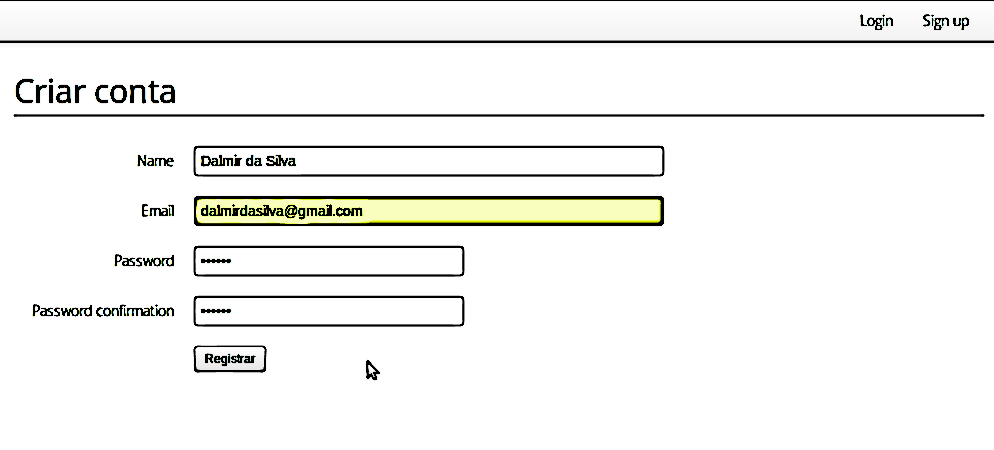
\includegraphics[width=.9\textwidth]{create_user.png}
        \caption{Protótipo de UI para UC01}
      \end{figure}

  \newpage

      \paragraph{UC02 - Autenticar usuário no sistema.} \hspace{10pt}

      \begin{table}[h]
        \begin{center}
          \begin{tabular}{ | p{7cm} | p{8cm} | }
            \hline
            Nome do UC: \cellcolor{gray} & Autenticar usuário no sistema. \\
            \hline
            Objetivo: \cellcolor{gray} & Autenticar um usuário existente no sistema. \\
            \hline
            Ativação: \cellcolor{gray} & Página principal / \em Login \\
            \hline
            \hline
            Cenário 1 - Autenticar um usuário: &  \\
            \hline
            Ação\cellcolor{gray} & Reação\cellcolor{gray} \\
            \hline
            Um usuário clica no \em link Login & O sistema exibe um formulário para o usuário entrar com as informações. \\
            \hline
            O usuário entra com os dados. E clica no botão 'Login'. & O sistema valida as informações. Autentica o usuário e redireciona para a página de lista de formulários. Em caso de falha, exibe mensagem de erro na tela. \\
            \hline
          \end{tabular}
          \caption{UC02 - Autenticar usuário no sistema.}
        \end{center}
      \end{table}

      \paragraph{Protótipo de UI para UC02} \hspace{10pt}
      
      \begin{figure}[h!]
        \centering
        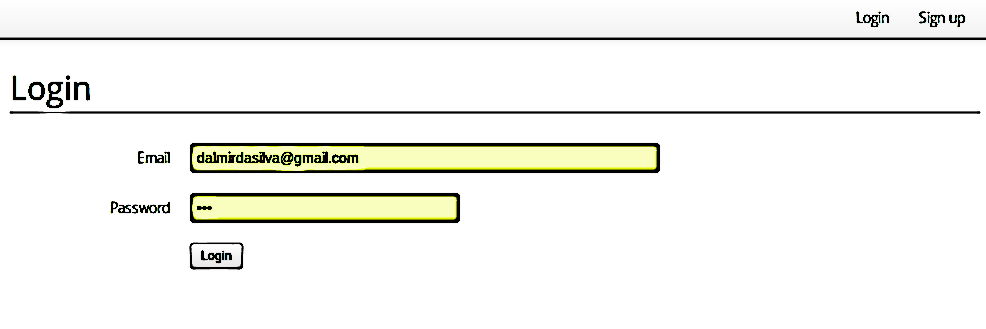
\includegraphics[width=.9\textwidth]{authenticate_user.png}
        \caption{Protótipo de UI para UC02}
      \end{figure}

      \paragraph{UC03 - Cadastrar formulário.} \hspace{10pt}

      \begin{table}[h]
        \begin{center}
          \begin{tabular}{ | p{7cm} | p{8cm} | }
            \hline
            Nome do UC: \cellcolor{gray} & Cadastrar formulário. \\
            \hline
            Objetivo: \cellcolor{gray} & Cadastrar um novo formulário no sitema. \\
            \hline
            Ativação: \cellcolor{gray} & Página principal / Meus formulários / Novo formulário \\
            \hline
            \hline
            Cenário 1 - Cadastrar um formulário: &  \\
            \hline
            Ação\cellcolor{gray} & Reação\cellcolor{gray} \\
            \hline
            Um usuário clica no botão 'Novo formulário' & O sistema exibe um formulário para o usuário entrar com as informações do novo formulário. \\
            \hline
            O usuário entra com os dasdos. E clica no botão 'Salvar'. & O sistema valida as informações, salva o formulário e redireciona para a página de edição do formulário. Em caso de falha, exibe mensagem de erro na tela. \\
            \hline
          \end{tabular}
          \caption{UC03 - Cadastrar formulário.}
        \end{center}
      \end{table}

      \paragraph{Protótipo de UI para UC03} \hspace{10pt}
      
      \begin{figure}[h!]
        \centering
        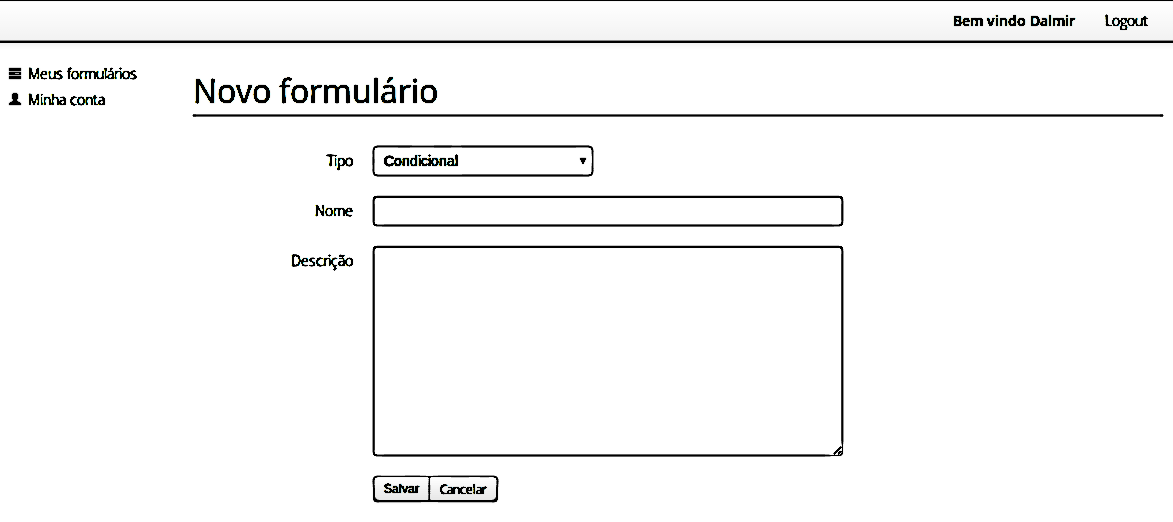
\includegraphics[width=.9\textwidth]{new_form.png}
        \caption{Protótipo de UI para UC03}
      \end{figure}

      \paragraph{UC04 - Editar formulário.} \hspace{10pt}

      \begin{table}[h]
        \begin{center}
          \begin{tabular}{ | p{7cm} | p{8cm} | }
            \hline
            Nome do UC: \cellcolor{gray} & Editar formulário. \\
            \hline
            Objetivo: \cellcolor{gray} & Editar um formulário existente no sitema. \\
            \hline
            Ativação: \cellcolor{gray} & Página principal / Formulário / Editor \\
            \hline
            \hline
            Cenário 1 - Editar um formulário: &  \\
            \hline
            Ação\cellcolor{gray} & Reação\cellcolor{gray} \\
            \hline
            Um usuário clica no botão 'Editor' & O sistema exibe as informações do formulário e uma lista de tipos de questão a ser adicionadas ao formulário. \\
            \hline
            O usuário clica no botão 'Adicionar', de um tipo específico de questão. & O sistema insere na tela um formulário para o usuário entrar com os dados da questão. Esse formulário deverá ser adicionado no final do formulário. \\
            \hline
            O usuário entra com o nome da questão e clica em salvar. & O sistema salva a questão, e exibe o feedback para o usuário. Sem recarregar a página. \\
            \hline
            O usuário pode repetir apartir da ação #2 quantas vezes desejar. &  \\
            \hline
          \end{tabular}
          \caption{UC04 - Editar formulário.}
        \end{center}
      \end{table}
      
      
      
      
      


      


  

  {\em Resenha sobre o artigo de Christiano O. Ávila, Rosana Silva e Luiz 
  A. Palazzo: {\bf Utilização de Sistemas Multiagentes na Contrução de Sistemas de Recomendação.}}
  \\\\

  Este artigo demonstra a utilização de Sistemas Multiagentes na 
  elaboração de uma ferramenta de recomendações chamada SisRecAC.
  \\

  Este sistema descobre e recomenda artigos científicos baseados em 
  documentos da própria pessoa que o utiliza. Através de agentes o sistema 
  descobre o conteúdo dos documentos atuas baseado em busca de 
  palavras-chaves e realiza pesquisa na base de artigos do Google, procurando
  por artigos similares.
  \\

  Assim que os novos artigos são encontrados, eles são exibidos para o 
  usuário que pode dar um {\em feedback}, informando o sistema a relevância 
  dos artigos encontrados. 
  \\

  Pode-se dizer que o principal objetivo do sistema é recomendar artigos 
  científicos que sejam similares a documentos armazenados no sistema ou 
  indicados pelos usuário.
  \\

  O sistema recebe os documentos do usuário, extrai as palavras-chaves e
  as utiliza na busca de novos artigos no Google Acadêmico. Para tal, os 
  sistema utiliza diferentes agentes com diferentes responsabilidades. 
  \\

  Existe um agente que é responsável pela extração de palavras chaves dos textos de entrada, 
  chamados de {\bf agente extrator}. Esse agente utiliza o critério de frequência 
  de ocorrências para classificar tais palavras, ele então, gera uma lista 
  das 'n' palavras mais frequêntes que serão usadas como critério de busca.
  \\

  Outro agente é responsável pela pesquisa e recolhimento de material baseados
  nas palavras-chaves encontradas do {\bf agente extrator}. Esse chama-se {\bf agente download}.
  \\

  Existem agentes responsáveis para realizar as conversões necessárias entre os 
  formatos dos documentos encontrados. Por exemplo, se o {\bf agente download} baixou um
  documento no formato do Word e o usuário gostaria de visualizar tal documento no formato
  de PDF, o agente {\bf doc 2 pdf} irá realizar a conversão do documento.
  \\

  Os agentes propostos buscam satisfazer a característica essencial da abordagem SMA que é
  a filosofia de resolução distribuída de problemas, utiliza a estratégia de dividir para
  conquistar. A resolução cooperativa distribuída de problemas diz que um problema é
  dividido em subproblemas e cada um é solucionado separadamente por um agente ou grupo
  de agentes, cada um destes comunicando ou cooperando entre si quando necessário, com a
  idéia básica de que a soma dos resultados locais corresponderá à solução do problema geral. 
  \\

  Desta forma é possível constatar que aplicar uma abordagem orientada à agentes para a
  resolução de um problema significa decompô-lo em múltiplos componentes autônomos
  com objetivos particulares e que se interrelacionam.
  \\

  \begin{center}
  \line(1,0){250}
  \end{center}

  Resenha sobre o artigo de Christiano O. Ávila, Rosana Silva e Luiz 
  A. Palazzo: {\bf Utilização de Sistemas Multiagentes na Contrução de Sistemas de Recomendação.}

\end{document}

